% Generated from paper/draft.md by paper/md2tex.py — edit the
% markdown and regenerate; do not hand-edit this file.
%
% Plain article class with a deliberately small package set: arXiv does
% not have your style files, and every package is a way for a remote
% compile to fail. Bibliography is inline (see md2tex.bibliography), so
% no BibTeX/Biber pass is required anywhere.
\documentclass[11pt]{article}
\usepackage[margin=1in]{geometry}
\usepackage{amsmath}
\usepackage{amssymb}
\usepackage{graphicx}
\usepackage{booktabs}
\usepackage[hidelinks]{hyperref}

% Figures live outside paper/ in the repo, but an arXiv bundle is flat.
% Naming them without a directory and listing both locations here means
% the same source compiles in-repo AND in a flattened submission.
\graphicspath{{../results/}{../out/}{./}}

\title{Holographic Scene Representation:\\Gaussian Splats as Hypervectors}
\author{Squatch Stack}
\date{}

\begin{document}
\maketitle
\begin{abstract}
A 3D Gaussian splatting scene is a list of primitives: fast to
rasterize, awkward to query, merge, or carry. We show that such a scene
can instead be \emph{superposed} into a single fixed-size complex
vector, and that three capabilities then follow from one algebra rather
than from three mechanisms. Encoding a point as $e^{iWp}$ with frequency
rows drawn from $\mathcal{N}(0, \Sigma^{-1})$ makes the inner product of
two encodings equal a Gaussian kernel, so a mixture of anisotropic
Gaussians is a random-feature bundle: evaluating the field anywhere is
an inner product, symbolic attributes attached by binding are recovered
by unbinding, an entire orthographic view folds into another vector of
the same kind, and independently-edited replicas merge by addition. A
single capacity law, $\sigma \sim \sqrt{N R / 2d}$, predicts the noise
of every one of those readouts and states where each stops working. We
demonstrate the representation on real captures of up to 682,000 splats,
evaluated against exact analytic ground truth rather than against
images, and we report the cost plainly: a bundle is roughly two orders
of magnitude larger than a modern splat codec at the same scene. The
contribution is not compression. It is that query, view synthesis, and
coordination-free merge become the \emph{same operation} on the same
object, with a measurable budget attached.
\end{abstract}

\section{Introduction}

3D Gaussian splatting~\cite{kerbl20233dgs} represents a scene as an
explicit collection of anisotropic Gaussian primitives, and that
explicitness is the source of both its speed and its awkwardness.
Rasterizing a list of primitives is fast. Asking a question of it ---
\emph{what is at this point?}, \emph{where are the objects labelled
``chair''?} --- means iterating the list. Merging two
independently-edited copies means reconciling two lists. Carrying a
scene means carrying every primitive.

Vector-symbolic architectures (VSAs) make composition algebraic:
structures are built by binding and bundling high-dimensional vectors,
and questions are answered by inverse operations rather than by
traversal. They are usually applied to symbols. The bridge to geometry
is fractional power encoding: representing a position $p$ as the
hypervector $e^{iWp}$ with frequency rows $w \sim \mathcal{N}(0,
\Sigma^{-1})$ makes the inner product of two such encodings equal the
Gaussian kernel
$\exp\!\left(-\tfrac{1}{2}(p-q)^{\mathsf{T}}\Sigma^{-1}(p-q)\right)$ ---
Bochner's theorem, in the form Rahimi and Recht~\cite{rahimi2007random}
made practical as random Fourier features and Frady et
al.~\cite{frady2021vfa} developed as Vector Function Architectures.

The consequence we build on is small to state and large in effect:
\textbf{a Gaussian splat mixture is already a random-feature bundle.}
Summing the encodings of N splats, weighted by their amplitudes,
produces one vector whose inner product with the encoding of any query
point returns the mixture's value there. The scene stops being a list.

This paper reports what that buys, what it costs, and where it fails.

\textbf{Three claims.}

1. \textbf{A splat scene is one vector, and queries are algebra.} With
importance-sampled mixture spectral codebooks, every splat keeps its own
anisotropic covariance inside a shared basis, and role-filler payloads
attached by binding answer attribute queries by unbinding. 2. \textbf{A
view is also just a bundle.} By the projection-slice theorem, folding
one per-frequency factor into the conjugate bundle turns an entire
orthographic render into another bundle of the same kind: every pixel is
one inner product, with no ray marching, no depth sort, and no geometry
present at render time. 3. \textbf{Superposition is almost a CRDT, and
the ``almost'' is exactly one axiom.} Bundling is commutative and
associative but not idempotent; two standard recipes close that single
gap and make holographic scene state mergeable without coordination.

\textbf{Two things we state up front rather than in a discussion
section.}

\emph{The boundary.} This is an emission --- tomographic ---
representation. Alpha compositing is non-linear and therefore outside
superposition's reach. We render X-ray projections and evaluate them
against analytic line integrals; we do not perform novel-view synthesis,
and we do not compete with rasterizers on photorealism.

\emph{The cost.} On the same capture, a holographic bundle is
approximately 400$\times$ larger and 50$\times$ less accurate at
reproducing the field than a current splat codec (\S7). If the task is
to store a scene and rasterize it later, the correct advice is to use
the codec. The claims above are about capabilities the codecs do not
provide, and the paper is written so that a reader can weigh that trade
with real numbers.

\section{Background}

\textbf{FHRR.} A hypervector is $d$ unit-magnitude complex phasors.
Binding is elementwise complex multiplication (phases add) and is
exactly invertible by the conjugate; bundling is addition; a fixed
random permutation tags order or role. Two independent random
hypervectors have similarity $0 \pm 1/\sqrt{2d}$, which is the noise
floor everything else trades against.

\textbf{Capacity as a contract.} Bundling N items puts crosstalk of
standard deviation $\sigma \sim \sqrt{N R / 2d}$ under every readout,
where R is the component power of what was bundled. Capacity is
therefore a signal-to-noise budget, never a table size, and structures
fail \emph{soft} --- noise, then errors --- rather than by allocation
failure. We treat this law as an API: every constructor documents its
budget, and every experiment reports measurement against prediction.

\textbf{Fractional power encoding.} Raising a hypervector to a real
power multiplies its phases, extending binding from a discrete operator
to a continuous one and giving the $e^{iWp}$ encoding above. Komer and
Eliasmith~\cite{komer2019fractional}'s Spatial Semantic Pointers develop
this for continuous space, including the shift
property~\cite{voelker2021ssp} we use in \S5.

\textbf{3D Gaussian splatting.}~\cite{kerbl20233dgs} A scene is a set of
anisotropic Gaussians with position, covariance, opacity, and
view-dependent colour, rendered by projecting and alpha-compositing them
front-to-back.

\section{Claim 1 --- A splat scene is one vector}

\subsection{Encoding}

The naive route --- one shared covariance for all splats --- fails
immediately on real data, where axis scales span five decades. We
instead store each splat's \emph{Fourier spectrum} sampled at a shared
random codebook, which keeps per-splat anisotropic covariance inside one
bundle at the cost of an importance-sampling variance penalty.

Drawing the codebook from a \textbf{mixture of Gaussians} spanning the
scene's scale range reduces that penalty from 16--33$\times$ to
2.4--3.2$\times$. Two rules were learned the expensive way, and both are
visible as structured artifacts rather than as noise when violated: the
finest mixture component must sit at the global scale floor, and
\emph{every} band's codebook must reach that floor --- because bands are
assigned by maximum axis scale, while a mid-band needle splat still has
thin axes at the floor. Violating the second rule paints herringbone
(Figure~\ref{fig:2}).

\begin{figure}[htbp]
\centering
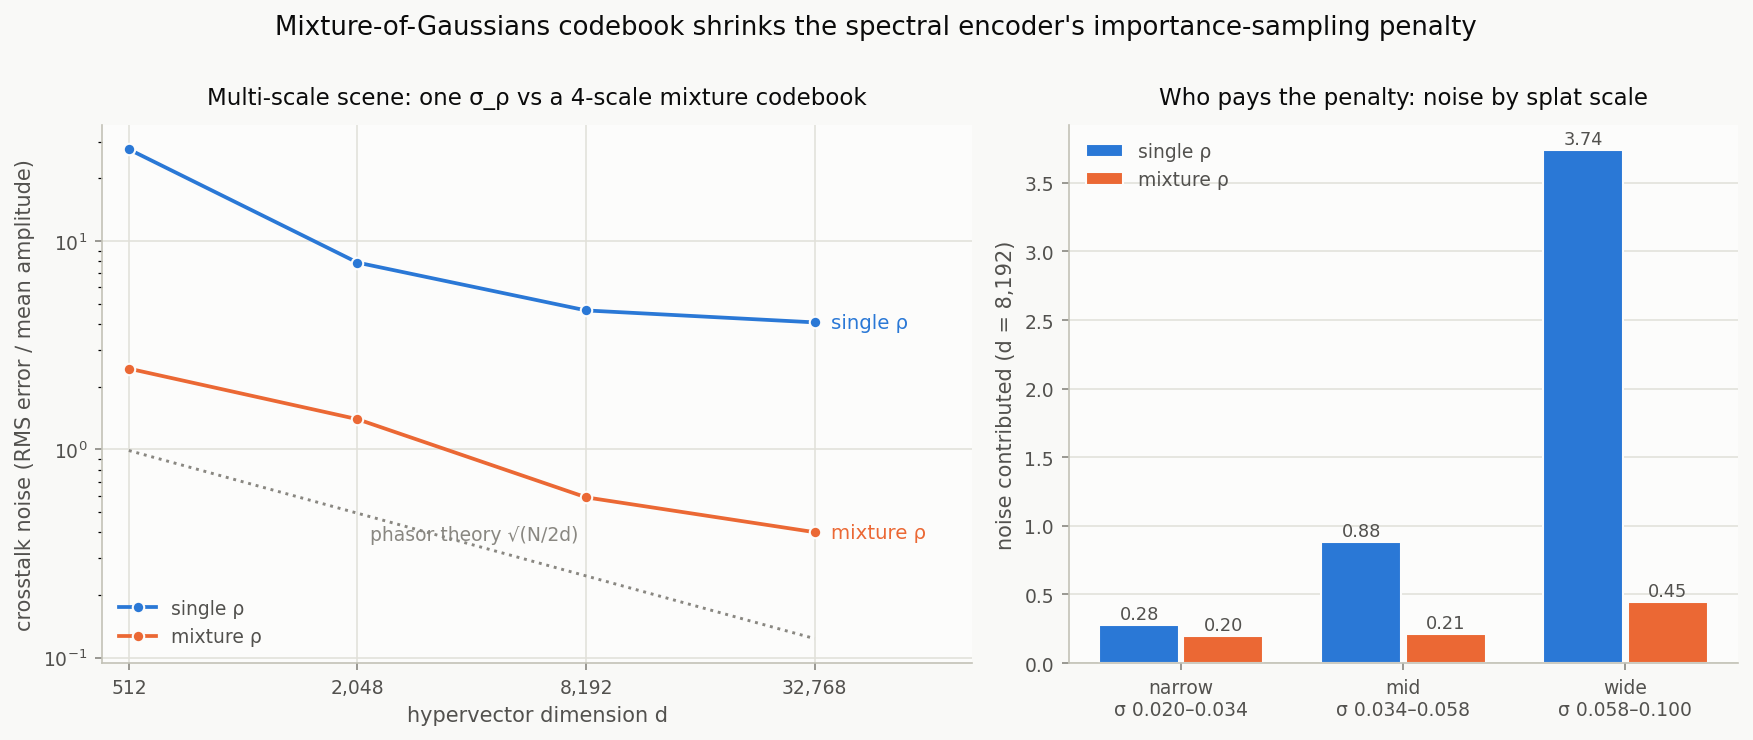
\includegraphics[width=\linewidth]{mog_penalty}
\caption{Why the codebook is a mixture. \emph{Left:} crosstalk noise against
hypervector dimension on a multi-scale scene, encoded against a single
shared frequency scale versus a four-scale mixture; the dotted guide is
the i.i.d. phasor prediction. \emph{Right:} which splats pay for it at d
= 8,192 --- the widest scale band contributes 3.74 with a single
codebook and 0.45 with the mixture. The mixture buys back
importance-sampling variance, not capacity.}
\label{fig:1}
\end{figure}

\begin{figure}[htbp]
\centering
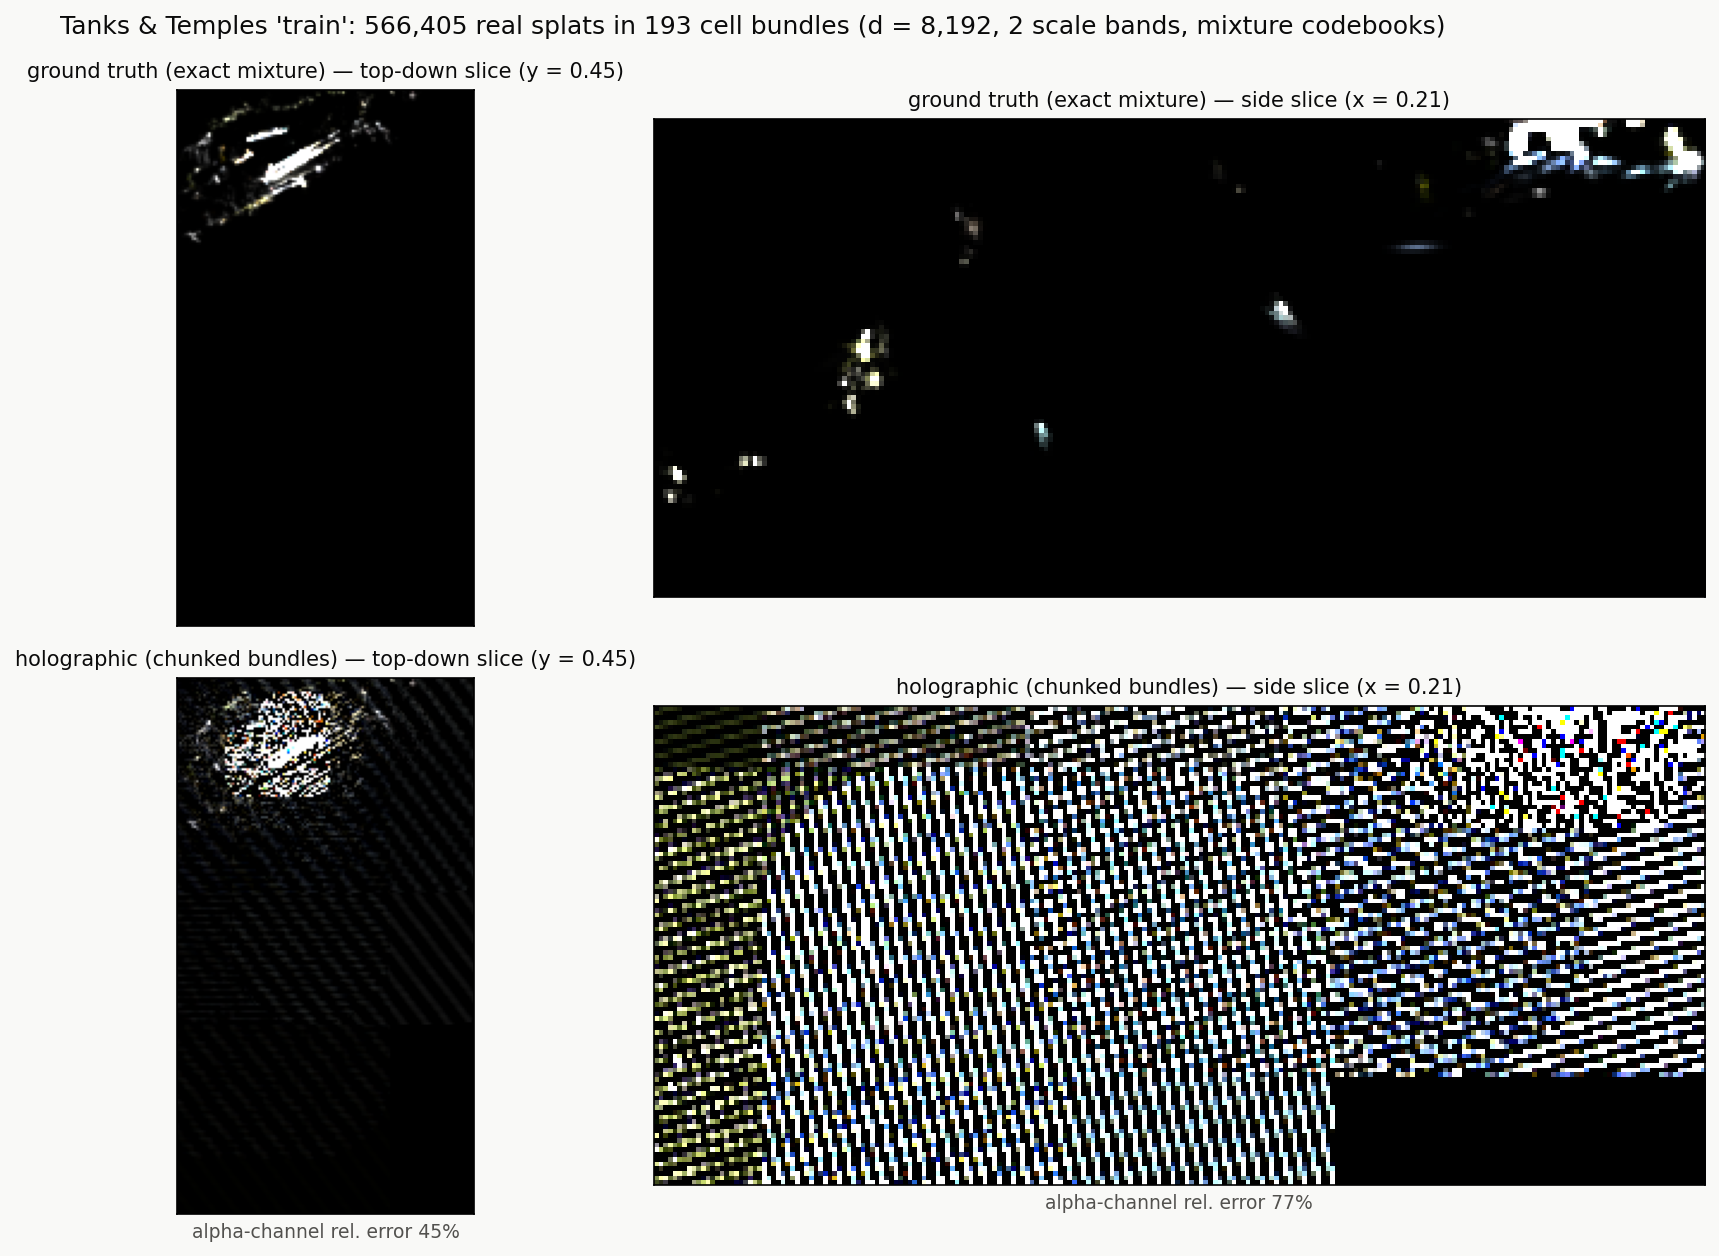
\includegraphics[width=\linewidth]{failure_herringbone}
\caption{The second codebook rule, violated: a band whose codebook does not reach
the global scale floor. The error is a structured herringbone rather
than noise, which is what makes the rule diagnosable by eye instead of
by metric.}
\label{fig:2}
\end{figure}

Real captures then require two more mechanisms. \textbf{Scale bands}
group splats by maximum axis scale, each band with its own codebook;
\textbf{spatial cells} chunk each band, so a query's crosstalk follows
\emph{local} density rather than N. Query reach follows the band's scale
cap, which is why splitting the finest band cut slice error by 33--44\%.

\subsection{Queries}

Evaluating the encoded field at a point is one inner product. Attaching
role-filler records to splats by binding, and recovering them by
unbinding, gives \texttt{what\_is\_at(p)} and \texttt{where\_is(label)}
directly --- the second returning a \emph{field} over space rather than
a list of matches. Because the codewords are hash-derived from
\texttt{(dim, seed)} rather than from sequential RNG state, any process
reconstructs them independently, which is what makes \S5 possible.

\subsection{Evidence}

Capacity curves fit $d^{-0.50}$ exactly, matching the law. Four real
captures --- two phone-scanned outdoor scenes, an indoor LiDAR cloud,
and a Tanks \& Temples scene, from 244k to 682k splats after cropping
--- pass through one fixed pipeline, and slices decode at 19\%/22\%
relative error against the \emph{exact Gaussian mixture} evaluated
cell-locally. Kernels agree across three compute backends to 2.5e-8.

\begin{figure}[htbp]
\centering
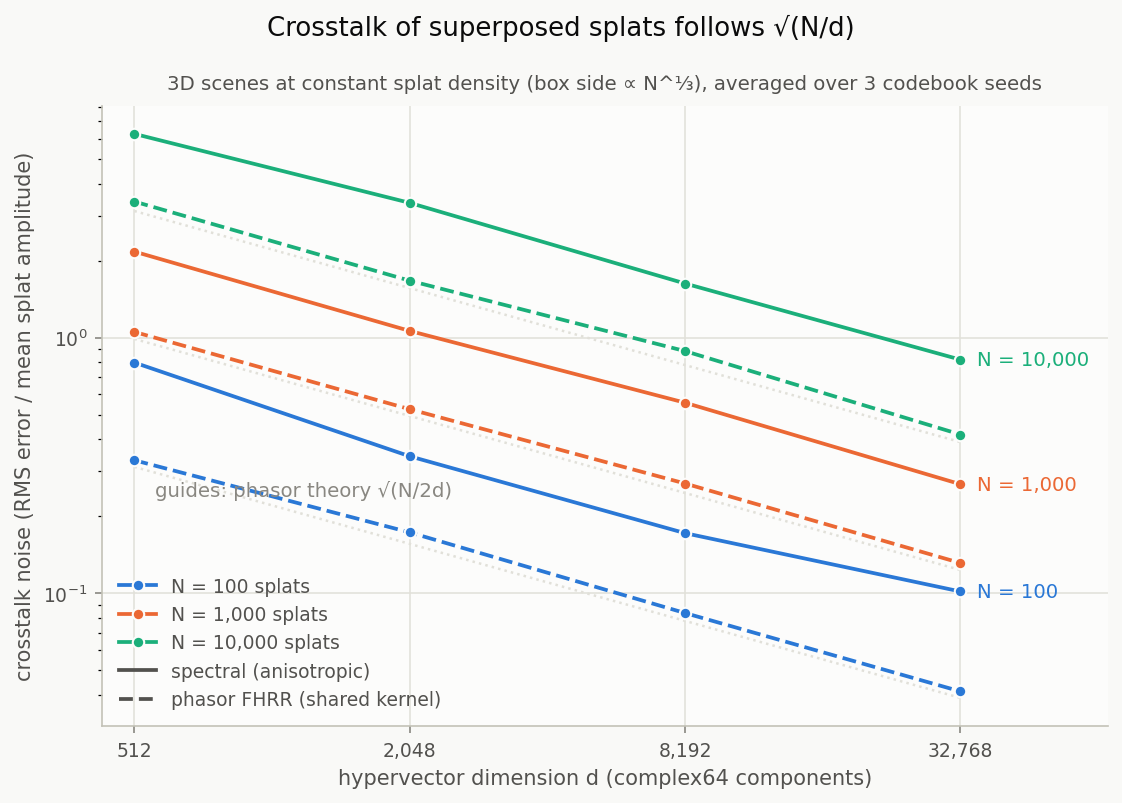
\includegraphics[width=\linewidth]{capacity_curve}
\caption{The law, measured. Crosstalk noise against dimension at constant splat
density for N = 100 / 1,000 / 10,000, comparing the anisotropic spectral
encoder (solid) against shared-kernel phasor FHRR (dashed); dotted
guides are the $\sqrt{\ }$(N/2d) prediction. Both families track the
law's d\textasciicircum{}(-1/2) slope over six octaves. The spectral
encoder sits above the guide by the importance-sampling penalty of
Figure~\ref{fig:1} --- the price of per-splat covariance.}
\label{fig:3}
\end{figure}

\begin{figure}[htbp]
\centering
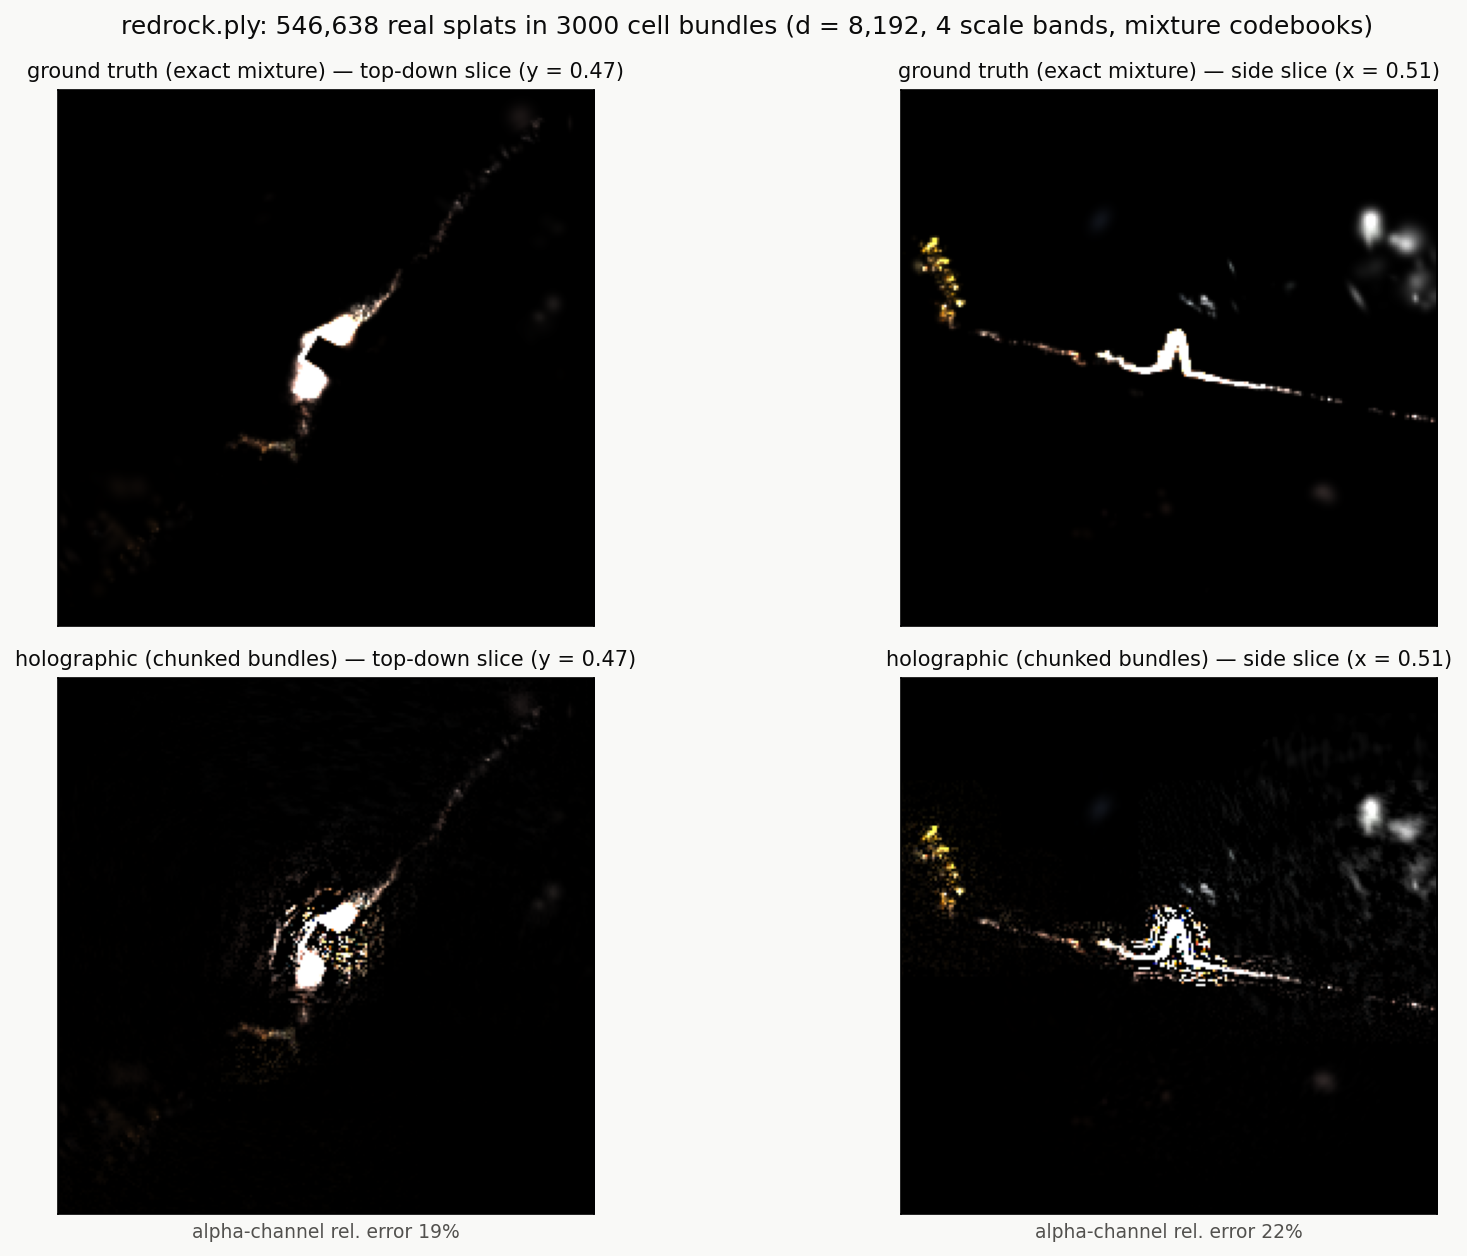
\includegraphics[width=\linewidth]{real_redrock}
\caption{Red Rock, the flagship capture: 547k splats after cropping, encoded
through scale bands and spatial cells, and scored against the exact
Gaussian mixture evaluated cell-locally. Three further captures --- a
second phone scan, an indoor LiDAR cloud, and a Tanks \& Temples scene
--- pass through the same fixed pipeline.}
\label{fig:4}
\end{figure}

\emph{Positioning.} VSA-OGM~\cite{snyder2024vsaogm} is the closest
published relative: SSP-encoded occupancy fields with sparse local
updates, but scalar occupancy only --- no per-splat covariance, colour,
rendering, learning, or replication. GVKF~\cite{song2024gvkf}
independently validates the ``splatting is a kernel mixture'' bridge
from the graphics side while keeping per-Gaussian parametric storage.

\section{Claim 2 --- A view is also just a bundle}

\subsection{Folding a view into the vector}

The bundle is the scene's Fourier transform sampled at random
frequencies. By the projection-slice theorem, the integral of the field
along a ray has a closed form in that domain: the ray integral depends
only on the spectrum in the plane perpendicular to the view direction.
Folding the corresponding per-frequency factor into the conjugate bundle
therefore turns an entire orthographic view into another bundle, and
every pixel becomes a single inner product against it.

There is no ray marching, no depth sort, and --- the part that surprises
people --- no geometry present at render time. The renderer's input is a
vector.

Because blur is covariance addition, mip levels are free: convolving the
scene with an isotropic Gaussian is adding $\sigma^2 I$ to every
covariance. This matters, because a projection uses only the spectrum
slice perpendicular to the view, so renders need their own dimension
budget; we encode a dedicated mip for rendering.

\subsection{Evidence}

On a synthetic 240-splat trefoil knot with analytic line integrals as
ground truth, views rendered from a single vector reach 5--7\% RMSE. On
real captures, a full turntable orbit is rendered entirely from 135 cell
bundles with no geometry at render time. Colour rides as amplitude on
one shared frequency basis, so RGB renders reuse the same phasors.

\begin{figure}[htbp]
\centering
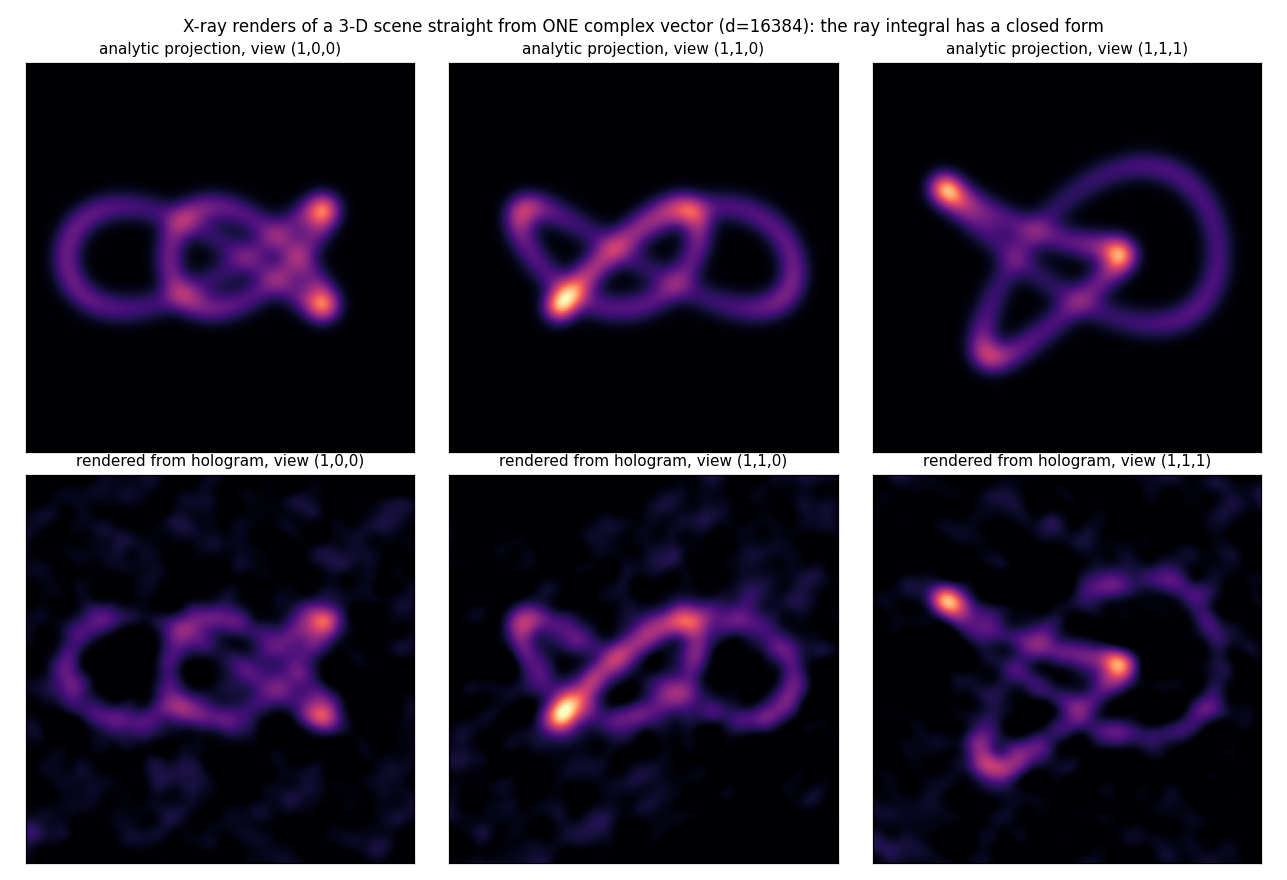
\includegraphics[width=\linewidth]{ray_render}
\caption{A view folded into the vector: the synthetic trefoil knot rendered from
a single bundle against analytic line integrals as ground truth, at
5--7\% RMSE. There is no ray marching, no depth sort, and no geometry
present at render time --- the renderer's input is a vector.}
\label{fig:5}
\end{figure}

\begin{figure}[htbp]
\centering
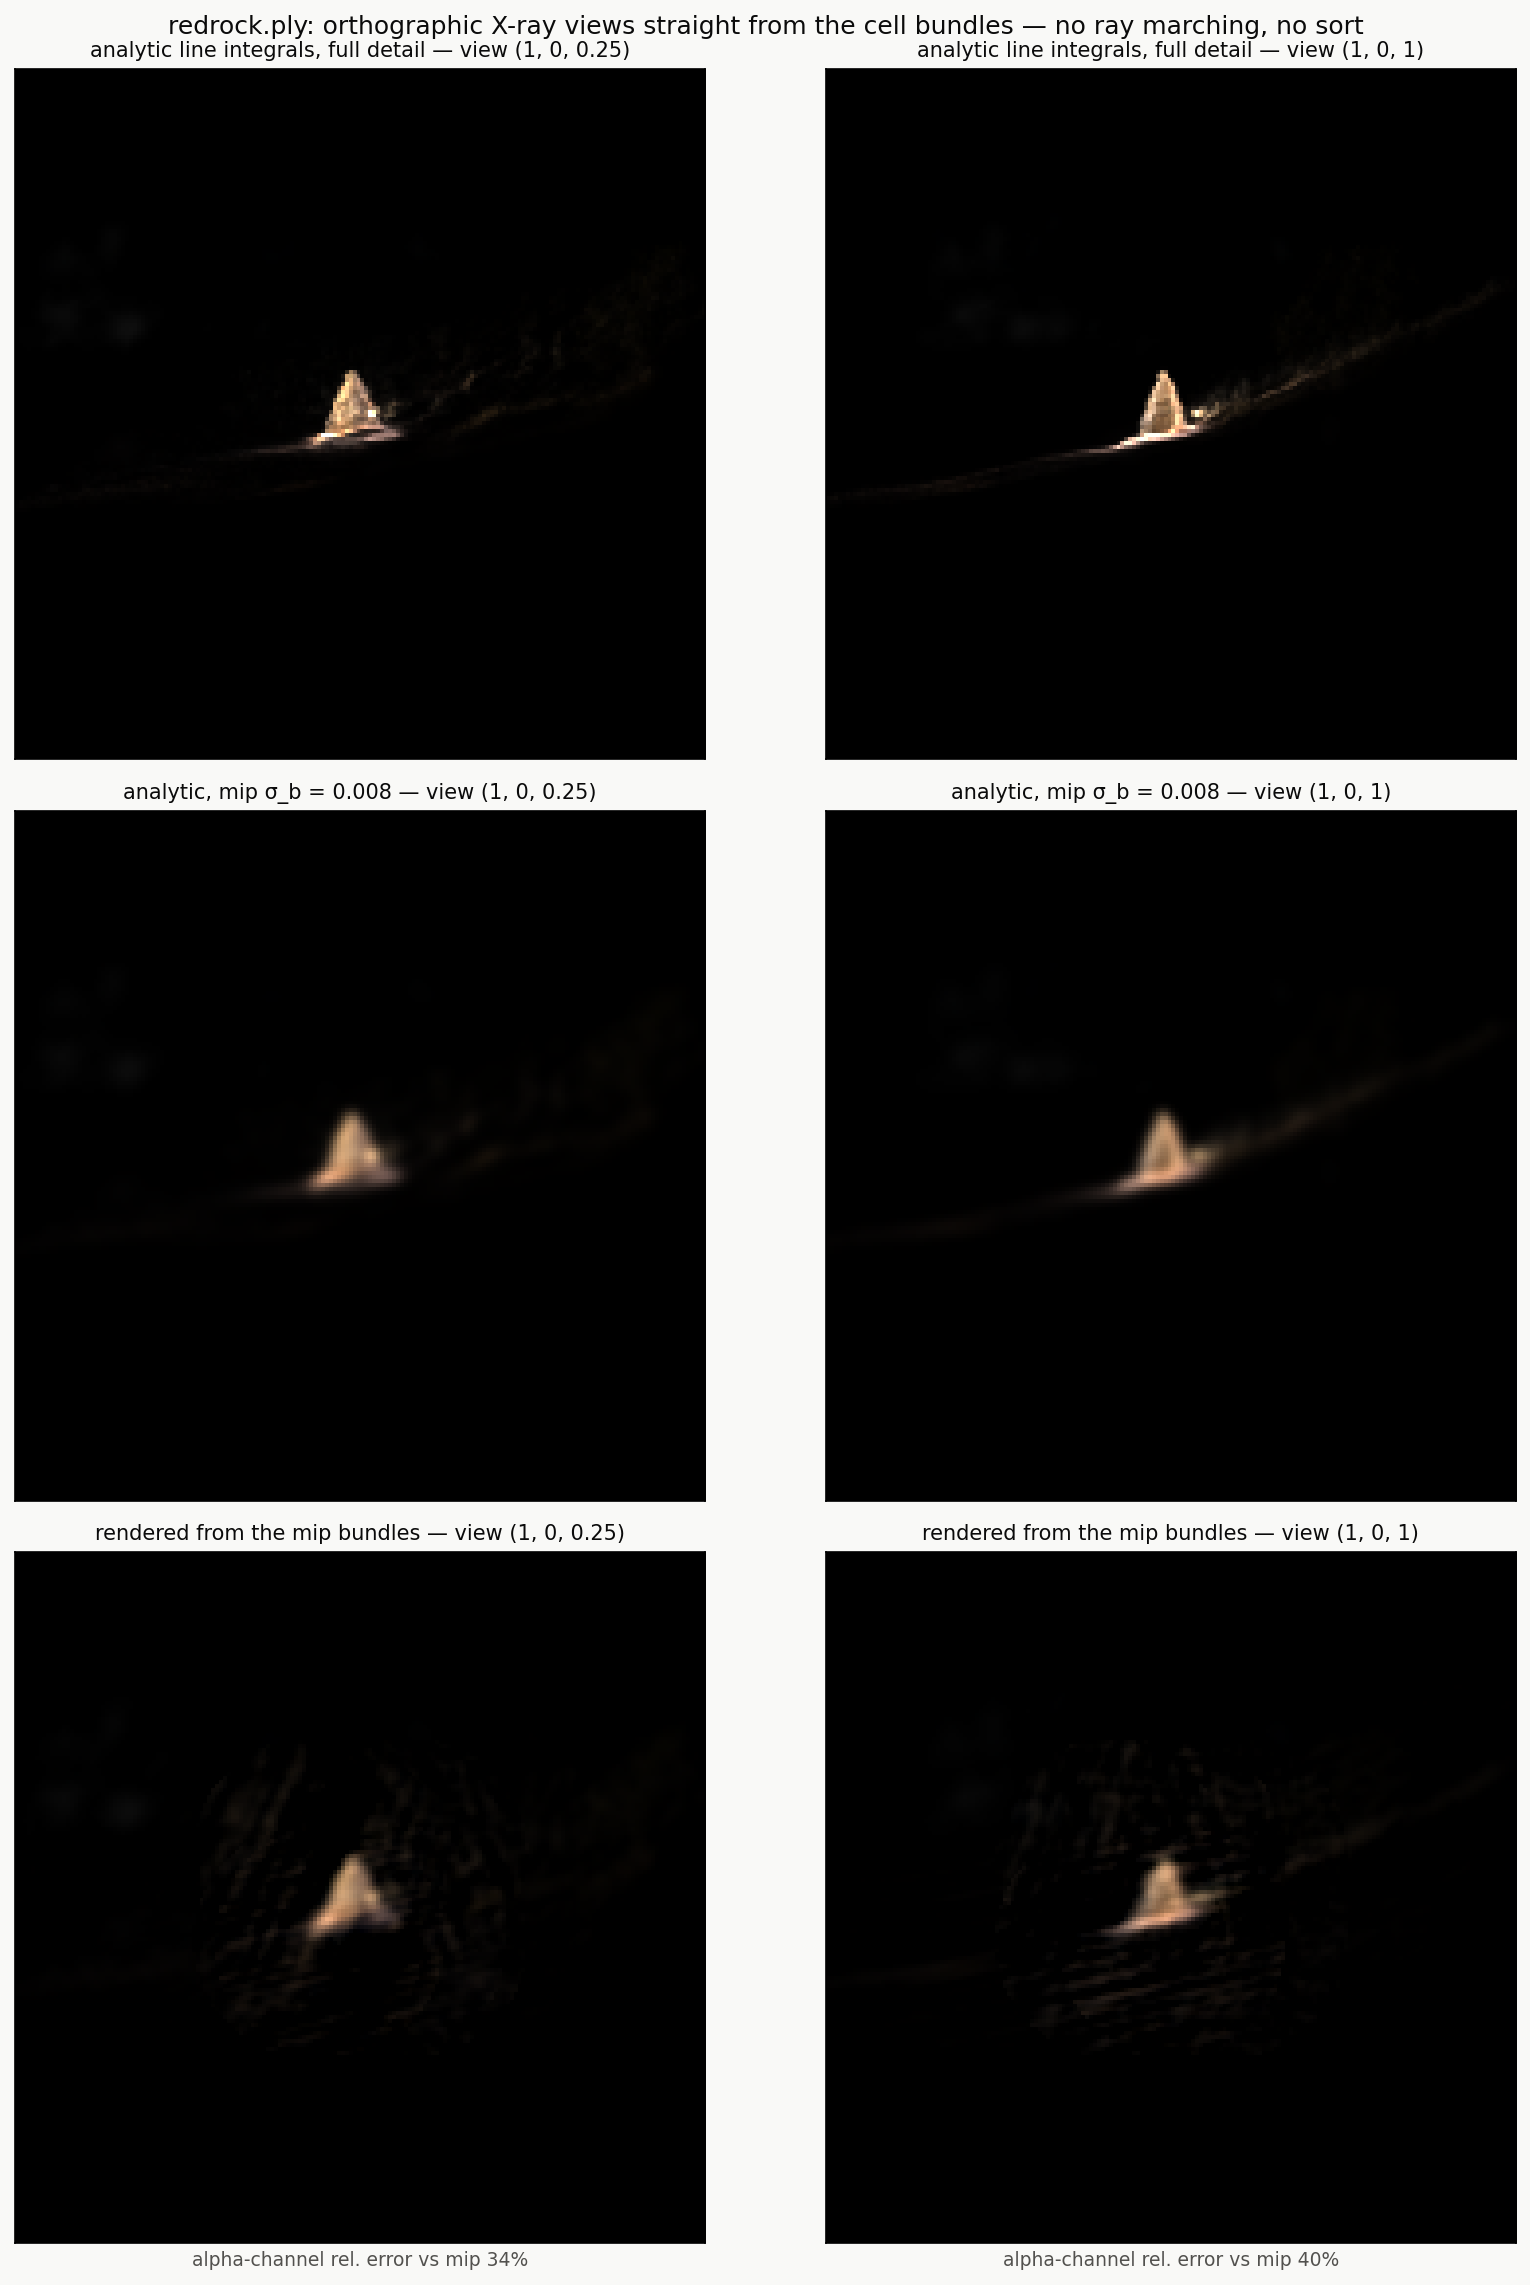
\includegraphics[width=\linewidth]{real_redrock_xray}
\caption{The same operation on real data: an X-ray view of Red Rock rendered from
cell bundles, against the analytic mip as referee.}
\label{fig:6}
\end{figure}

\subsection{The boundary, stated as a result}

Emission and tomography only. Occlusion requires ordering and
compositing, which are non-linear operations that superposition does not
admit. We consider this worth stating precisely rather than hedging: the
representation renders what integrates, and a scene where visibility
matters needs a compositing pass outside the algebra.

\emph{Positioning.} CryoSplat~\cite{chen2025cryosplat} and
R2-Gaussian~\cite{zha2024r2gaussian} both exploit the Fourier slice
theorem for closed-form Gaussian projection --- per primitive. Folding a
whole \emph{view} into one random-feature vector appears to be new.

\section{Claim 3 --- Superposition is almost a CRDT}

\subsection{The one missing axiom}

A conflict-free replicated data type requires a merge that is
commutative, associative, and idempotent. Bundling --- vector addition
--- is trivially commutative and associative. It is not idempotent:
adding the same contribution twice double-counts it, so redelivered
updates corrupt state.

That single gap has a standard fix. Each writer accumulates only its own
bundle, and the merged hologram is the sum over writers, so redelivery
is absorbed by the underlying delta protocol's version vectors. Merges
are then bit-identical on every replica that has seen the same updates.

Deletion is subtler. Subtracting a contribution has PN-counter
semantics, and two peers concurrently retracting the same item
over-cancel into a \emph{negative phantom}. Changing the type of the
operation fixes it: removals become tombstones in a grow-only set, the
subtraction is derived once by every reader, concurrent duplicate
removal is idempotent, and a concurrent re-add wins because it carries a
fresh identifier the remover never observed.

Determinism is what makes all of this coordination-free. Codewords and
frequency matrices are hash-derived from \texttt{(dim, seed)}; a
codebook built from sequential RNG state would assign vectors by
creation order and replicas would silently disagree.

\subsection{Evidence}

Two peers paint halves of a scene offline and delta-sync into one, with
matching state and render digests; attributed scenes merge with labels
riding a grow-only registry, so a peer answers queries for labels it
never used locally. A two-process demonstration exchanges only
length-prefixed deltas over TCP and includes the adversarial case: both
painters concurrently undo the same stroke, which is tombstoned twice
and subtracted once.

\begin{figure}[htbp]
\centering
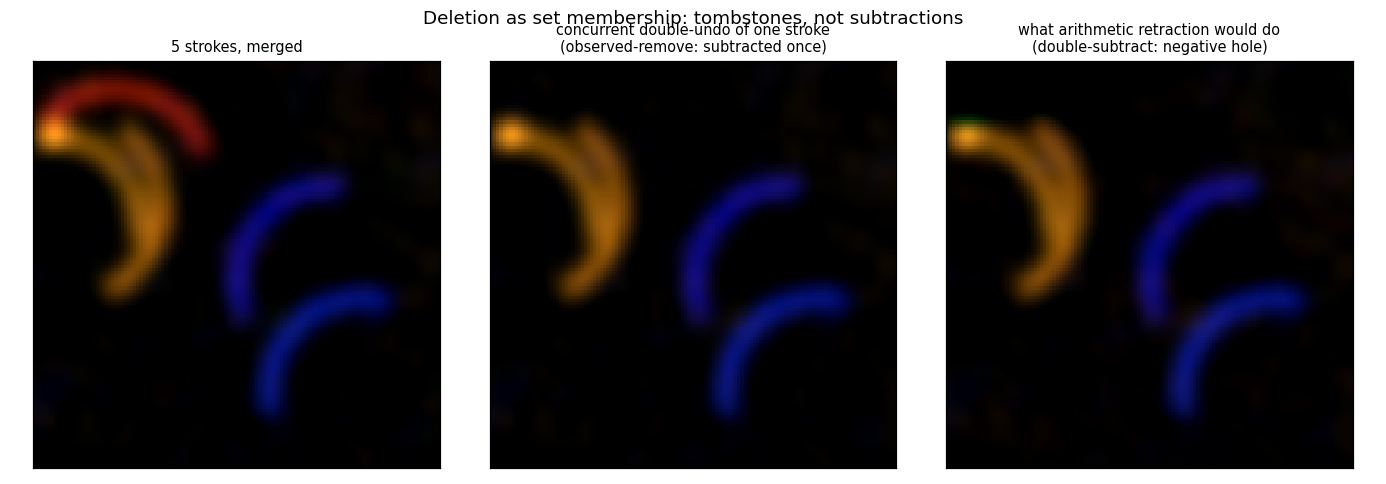
\includegraphics[width=\linewidth]{orset_undo}
\caption{Why deletion is set membership rather than arithmetic. \emph{Left:} five
strokes, merged. \emph{Centre:} both peers concurrently undo the same
stroke under observed-remove semantics --- tombstoned twice, subtracted
once, and the stroke is simply gone. \emph{Right:} what arithmetic
retraction does instead --- the contribution is subtracted twice and
leaves a negative phantom where the stroke was.}
\label{fig:7}
\end{figure}

\begin{figure}[htbp]
\centering
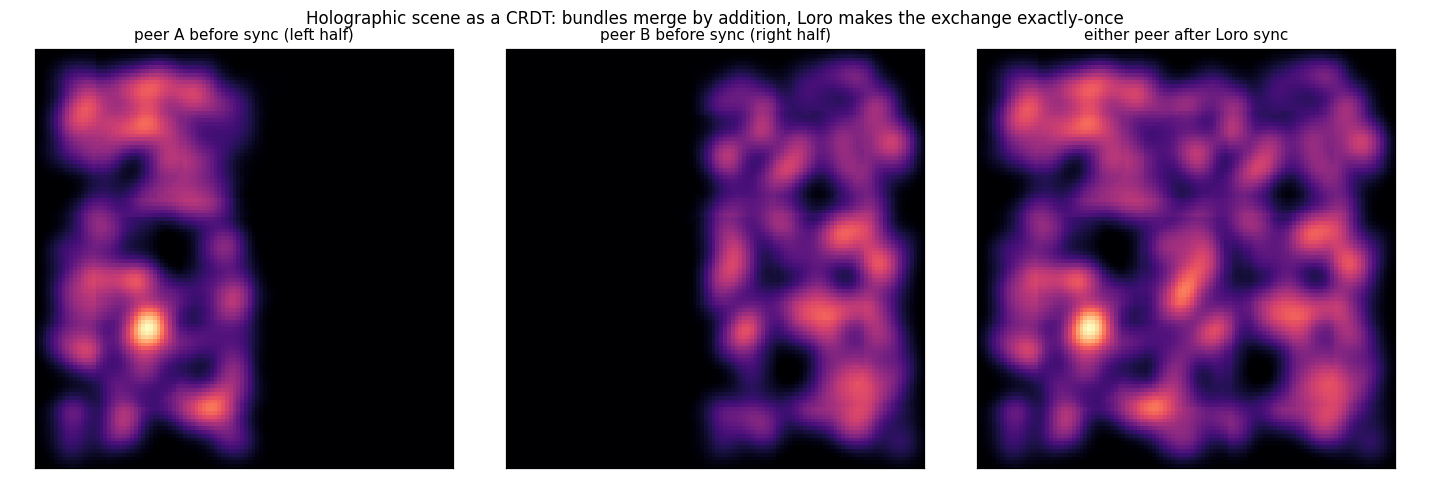
\includegraphics[width=\linewidth]{crdt_scene}
\caption{Two peers paint halves of a scene offline and delta-sync into one,
reaching matching state and matching render digests. Merge is addition;
the coordination is in the delta protocol, not in the representation.}
\label{fig:8}
\end{figure}

\emph{Positioning, and a contrast.} Recent work wrapping neural-network
model merging~\cite{gillespie2026crdtmerge} in CRDT semantics reports
that all 26 merge strategies tested --- weight averaging, SLERP, TIES,
DARE, Fisher, evolutionary --- fail commutativity, associativity, or
idempotency. Superposition satisfies the first two by construction and
fails only the third. The recipes above close that one gap, which is a
cheaper starting position than the merging literature usually enjoys.

\section{The law, and where it bends}

Section 2 states the capacity law; this section is where it is tested
rather than asserted. Every demonstration in this work prints its
measured curve beside the prediction, and the agreement is close enough
that the interesting content is in the four places where it is not. Each
deviation is a case where an assumption behind the i.i.d. law fails, and
each names either its remedy or its open problem.

\textbf{Dense scenes correlate their noise.} The law assumes bundled
items are independent. Splats that sit near each other in a dense
capture are not: they share frequencies, and their crosstalk adds
coherently rather than in quadrature, inflating $\sigma$ by roughly
1.5--3$\times$ over prediction. The practical consequence is that the
obvious remedy does not work. If the residual were Monte-Carlo noise,
more dimensions would wash it out --- so we doubled $d$ on the densest
capture and measured the result: a 2--4\% improvement for 600 MB of
additional storage. That negative result is what identifies the error as
coherent, and it redirects the problem from ``spend dimensions'' to
``decorrelate or denoise'', which we return to in \S9.

\textbf{Fitting is sampling-limited at real density.} Because the
readout is linear in the bundle, the bundle is literally the weight
vector of a random-feature regression, and it can be \emph{fitted} to
samples rather than accumulated from splats. On synthetic mixtures this
is dramatic: the fitted vector beats the forward-encoded one by roughly
70$\times$ in held-out error, because regression finds the optimal
vector in the same basis and corrects crosstalk that forward bundling
simply carries. On real captures it loses (0.72/0.53 against forward
encoding's 0.52/0.38).

\begin{figure}[htbp]
\centering
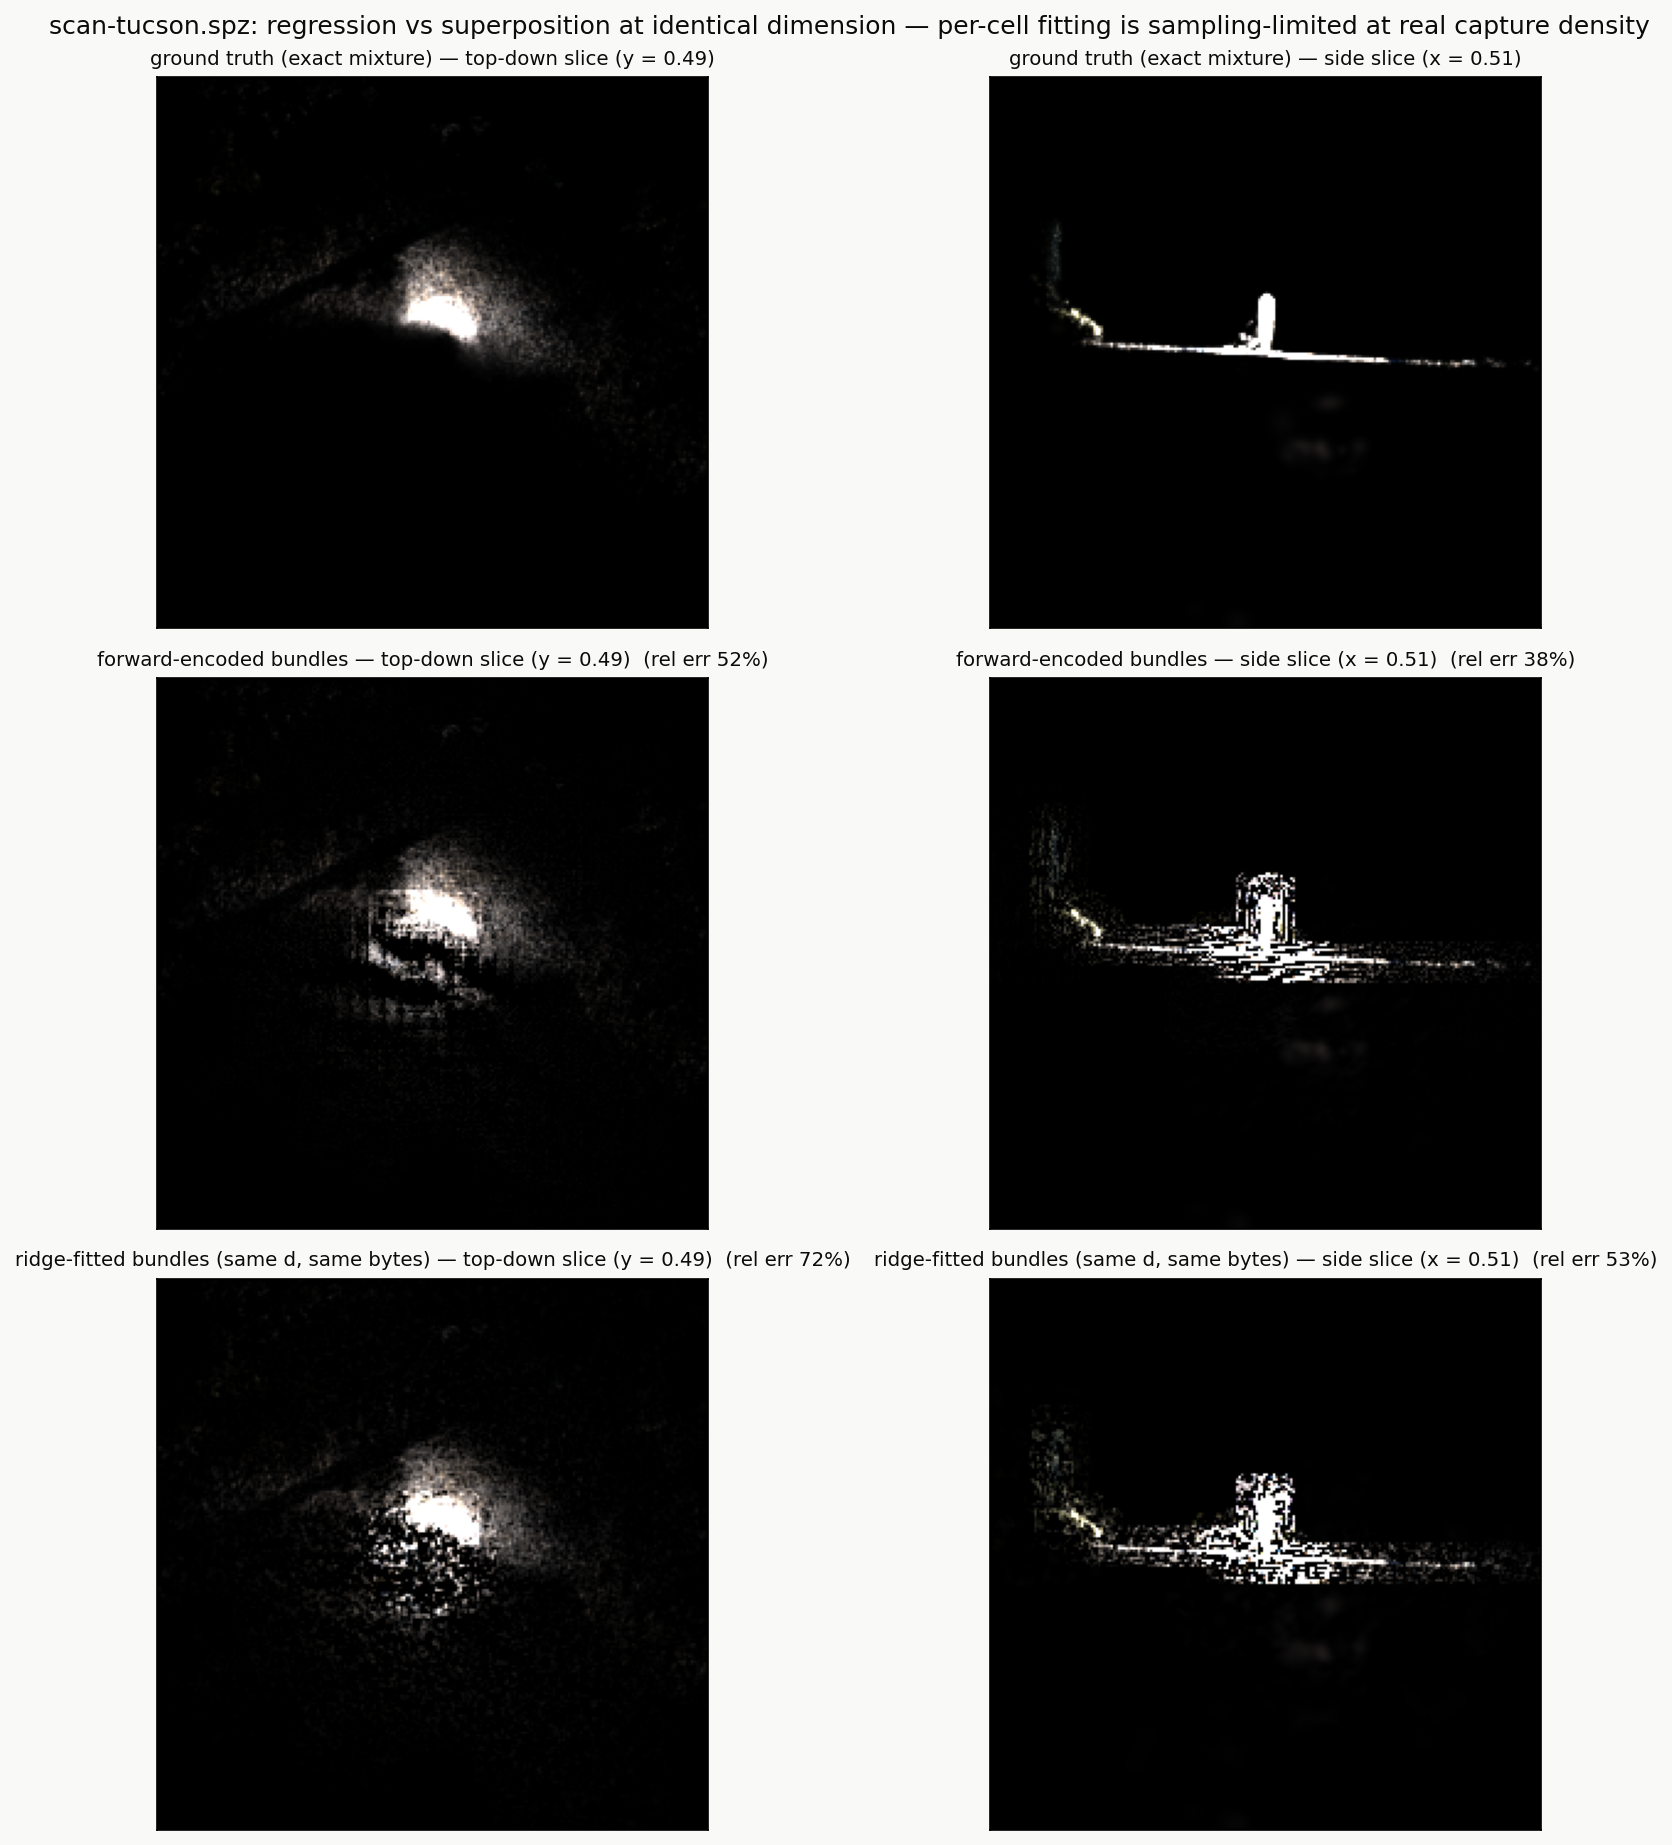
\includegraphics[width=\linewidth]{real_fit}
\caption{Fitting loses at real capture density. Top-down and side slices of
scan-tucson: the exact mixture (top), forward-encoded bundles (middle,
52\% / 38\%), and ridge-fitted bundles at identical dimension and
identical bytes (bottom, 72\% / 53\%). On synthetic mixtures the
ordering is reversed by roughly 70$\times$; what changes is sample
coverage, not the method.}
\label{fig:9}
\end{figure}

The diagnosis is coverage: hundreds of floor-scale splats per cell need
samples at their own kernel width, which is tens of thousands of samples
per cell, beyond what the dual solve can absorb. A spectral prior was
necessary even to make the fit competitive --- without it, minimum-norm
regression spreads energy into the codebook's finest frequencies and
memorizes samples as kernel-width bumps, twelve times worse than forward
encoding. The natural next step, a zero-sample analytic projection with
a closed-form region Gram, lands inside the classical
Fourier-extension~\cite{adcock2012fourier} problem: severely
ill-conditioned, but provably stable under regularized least squares,
which tells us the route needs Tikhonov or truncated-SVD treatment from
the first line rather than as a rescue.

\textbf{The scale floor is radiometric, not merely geometric.} Encoding
imposes a resolution floor on axis scales, and real captures hit it
constantly --- 99.4--99.7\% of encoded splats in every Gaussian capture
we tested have a thin axis pinned to it, because 3DGS splats are
overwhelmingly needle-shaped. Raising a thin axis while holding peak
amplitude fixed raises that splat's integral, and across one capture the
floor inflates total scene mass by 11$\times$. Quantifying what this
costs turns out to be a trap worth documenting: measured by point
sampling, the answer is meaningless, because a sheet thinner than the
sampling grid is nearly invisible to point evaluation regardless of how
much mass it carries. Integrating over a pixel footprint instead is
exact and cheap --- a Gaussian convolved with a Gaussian is a Gaussian,
so covariances simply add --- and against a footprint-integrated target
the pipeline reports 11.5\% where the sharp-against-sharp pair reports
18.1\%. The lesson generalizes past this system: the referee has to
measure the same field the representation was asked to encode.

\textbf{Storage has a rate-distortion boundary at magnitude.} Phase-only
codes, which store each dimension's angle and discard its length, floor
amplitude-carrying fields at roughly 0.24 relative RMSE at \emph{any}
bit depth. The reason is structural rather than numerical: a bundle
accumulated from weighted contributions carries information in its
magnitudes, and a unit-magnitude code throws that away before the first
bit is allocated. Magnitude-preserving codes cross the boundary, and a
gamma-companded polar code is the faithful choice for the
wide-dynamic-range bundles real captures produce. Recent independent
work on quantized-phase FHRR~\cite{snyder2026qfhrr} reaches the same
boundary from the opposite side: its bundling operation is not closed
under phase quantization and must project back onto the unit circle,
discarding exactly the magnitude our measurements identify as necessary.

\begin{figure}[htbp]
\centering
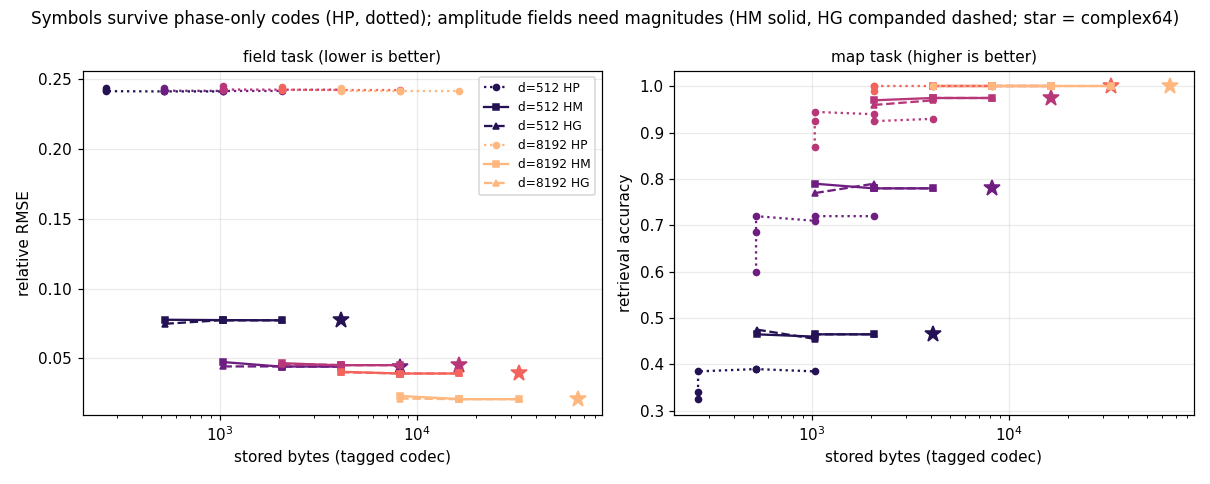
\includegraphics[width=\linewidth]{codec_curve}
\caption{The rate-distortion boundary is structural, not a bit depth. \emph{Left,
field task:} phase-only codes (HP, dotted) sit on a flat error floor no
matter how many bytes are spent, while magnitude-preserving codes (HM
solid, HG companded dashed) fall well below it; stars mark uncompressed
complex64. \emph{Right, map task:} for codeword retrieval, where
magnitude carries nothing, the same phase-only codes are competitive at
a fraction of the bytes. One representation, two tasks, opposite
verdicts --- which is the whole of the codec split.}
\label{fig:10}
\end{figure}

Taken together these four say something more useful than any of them
alone. The law is not a decoration: it predicts well enough that its
failures are informative, and every failure here was found by measuring
against it rather than by noticing an artifact.

\section{What it costs}

A representation should be judged by a referee it did not choose. We
score every candidate identically: reconstruct the field it encodes,
evaluate that field at the same query points, and compare against the
exact Gaussian mixture of the source capture. Per-splat formats lose to
quantization, holographic bundles lose to crosstalk, and the referee is
indifferent to which.

\begin{table}[htbp]
\centering
\begin{tabular}{lrrr}
\toprule
representation & MB & bytes/splat & field error \\
\midrule
PLY (SH degree 0) & 3.9 & 85 & 0.0\% \\
SPZ v3 & 1.0 & 22 & 0.0\% \\
SOG (SH palette) & 0.8 & 18 & 0.3\% \\
holographic bundles (d = 8,192) & 382.8 & 8,354 & 17.4\% \\
same, 8-bit magnitude codec & 95.7 & 2,089 & 17.0\% \\
same, 4-bit magnitude codec & 47.9 & 1,045 & 25.8\% \\
\bottomrule
\end{tabular}
\end{table}

The result is a loss, and reporting it precisely is the point of running
the experiment. A bundle is approximately 400$\times$ larger and
50$\times$ less accurate at reproducing the field than a current splat
codec. A reader whose problem is to store a scene and rasterize it later
should use the codec; nothing in this paper argues otherwise.

What the bytes buy is the subject of \S\S3--5: query by algebra rather
than by traversal, an entire view as a second vector of the same kind,
and merge by addition with no coordination. A codec sells none of those,
and sells bytes extremely well.

Two observations survive the loss. The first is that the 8-bit magnitude
codec is \emph{free}: four times smaller at slightly better error than
the uncompressed bundle. Max-scaled quantization zeroes the smallest
components, and on a forward-encoded bundle those components are mostly
crosstalk, so the codec acts as an accidental shrinkage denoiser.
Pushing to 4 bits finally costs accuracy, which places the useful
operating point at 8.

The second is that the two families scale differently with density.
Bundle bytes are fixed per occupied cell however many splats fall inside
it, while every per-splat format grows linearly with content. Holding
the scene volume fixed and increasing splat count tenfold costs a codec
10$\times$ and costs bundles 2.6$\times$, narrowing the gap fourfold per
decade. Honesty requires the other half of that sentence: the gap
narrows but does not close at any density a real capture produces. The
useful form of the claim is about shape rather than crossover ---
per-splat formats scale with detail, bundles scale with occupied volume,
so a bundle's cost is predictable from a scene's extent before its
contents are known.

\section{Related work}

\textbf{Foundations.} The algebra is Plate's Holographic Reduced
Representations~\cite{plate1995hrr,plate2003hrr} in its Fourier form,
with Kanerva's Sparse Distributed
Memory~\cite{kanerva1988sdm,kanerva2009hdc} as the ancestor of the
capacity-as-signal-to-noise framing. The bridge from that algebra to
continuous geometry is fractional power encoding, developed as Vector
Function Architectures by Frady et al.~\cite{frady2021vfa} and as
Spatial Semantic Pointers by Komer and
Eliasmith~\cite{komer2019fractional}; the kernel identity it relies on
is Bochner's theorem in the practical form Rahimi and
Recht~\cite{rahimi2007random} introduced as random Fourier features.
Kleyko et al.'s surveys~\cite{kleyko2021survey1,kleyko2021survey2} are
the field's own account of what is settled.

\textbf{Work that bounds these claims.} Four results remove things this
paper might otherwise have claimed, and we adopt each rather than
rediscover it. Quantized-phase FHRR~\cite{snyder2026qfhrr} with
integer-only binding is published: our phase codec is that
representation reached from storage rather than from hardware, so we
claim only the measured boundary where it fails and not the
representation itself. Anti-aliasing in Gaussian splatting is solved by
constraining primitive size to the input views' sampling
rate~\cite{yu2024mipsplatting} and by integrating over the pixel window
analytically~\cite{liang2024analytic}; our resolution floor is an ad-hoc
version of the former, and our footprint evaluator is the pre-projection
form of the latter. Trajectory simulation via the shift
property~\cite{voelker2021ssp} of fractional binding already exists for
single and multiple objects, so translation as a phase ramp is not a
contribution of this work. And recent work wrapping neural-network model
merging~\cite{gillespie2026crdtmerge} in CRDT semantics is the nearest
neighbour to \S5 --- different object, same shape, and the source of our
sharpest contrast.

\textbf{Nearest neighbours.} VSA-OGM~\cite{snyder2024vsaogm} is the
closest published relative overall: SSP-encoded occupancy fields with
sparse local updates, achieving large latency and memory wins over dense
baselines, but representing scalar occupancy only --- without per-splat
covariance, colour, rendering, learning, or replication.
GVKF~\cite{song2024gvkf} arrives at the ``splatting is a kernel
mixture'' bridge from the graphics side while retaining per-Gaussian
parametric storage. CryoSplat~\cite{chen2025cryosplat} and
R2-Gaussian~\cite{zha2024r2gaussian} both apply the Fourier slice
theorem to Gaussian primitives for closed-form projection, per primitive
rather than per view. HyperSpace~\cite{snyder2026hyperspace} is the
nearest VSA-framework effort and contains no scene, splat, or
replication content.

\textbf{Graphics.} Rasterization is better at rasterizing, and the
compression literature~\cite{ali2025compression} this work is measured
against in \S7 is better at compression. The contribution here is not a
faster or smaller renderer; it is that a scene, a view of it, and a
merge of two edits to it are the same kind of object, with one budget
that predicts the error of each.

\section{Limitations and future work}

The hard limit is occlusion. Alpha compositing requires ordering and
non-linear accumulation, neither of which superposition admits, so the
representation renders what integrates. A hybrid --- holographic density
with a classical compositing pass --- is the obvious shape of a solution
and remains unexplored.

Storage is large in absolute terms, as \S7 quantifies. Rotation is not a
phase ramp: translation is exactly a phase ramp, but rotation remixes
frequencies across the codebook and needs a mechanism of its own.
Determinism is semantic rather than bitwise --- recomputed vectors agree
to about a part in 10$^7$, far under any decision threshold, but digests
must hash transmitted bytes rather than recomputed sums. Banded and
clustered readout strategies pay off only when the data has structure to
exploit: spatial locality for scenes, and its analogue elsewhere.

The open directions follow the deviations in \S6. The coherent
dense-scene residual needs a denoiser rather than more dimensions, and
the accidental shrinkage observed in \S7 suggests that deliberate
thresholding at the crosstalk noise level is the first thing to try. The
zero-sample analytic projection needs regularization from the start for
the reasons the Fourier-extension~\cite{adcock2012fourier} literature
gives. Dynamic scenes are the natural extension of \S5's mergeable
state, with the caveat that the underlying shift mechanism is
established work and only the capture-scale combination would be new.

One result belongs here as evidence of generality rather than as a
claim. The same capacity law and the same partition-plus-locality remedy
transfer intact from geometric scenes to \emph{rule tables}, where a
similarity-dispatch engine over messy text reaches 0.98 accuracy at
43$\times$ less compute than exhaustive matching, and fails in exactly
the way the law predicts when its budget is exceeded. That the law
governs a domain containing no geometry is the strongest evidence
available that it is a property of superposition rather than of splats.

\section{Conclusion}

A 3D Gaussian splatting~\cite{kerbl20233dgs} scene can be superposed
into a single fixed-size complex vector, and once it is, three
capabilities stop being separate mechanisms. Evaluating the scene is an
inner product. Rendering an orthographic view of it is folding one
factor into that vector and taking more inner products. Merging two
independently edited copies is addition, needing only the single missing
axiom to be supplied. One capacity law predicts the error of all three
and, more usefully, predicts well enough that its four failures are
diagnostic.

The cost is real and we have measured it: two orders of magnitude more
storage than a modern splat codec, at fifty times the error, for a
representation that does not composite and therefore does not render
what a rasterizer renders. What it offers in exchange is that a scene
becomes an object with an algebra --- one where a query, a view, and a
merge are the same operation applied differently, and where the noise
budget of each is known before it is run.

\begin{thebibliography}{22}

\bibitem{plate1995hrr}
Tony A. Plate.
\newblock Holographic Reduced Representations.
\newblock \emph{IEEE Transactions on Neural Networks}
\textbf{6}(3):623--641, 1995.
\newblock \texttt{doi:10.1109/72.377968}.

\bibitem{plate2003hrr}
Tony A. Plate.
\newblock Holographic Reduced Representation.
\newblock \emph{CSLI Publications}, 2003.

\bibitem{kanerva1988sdm}
Pentti Kanerva.
\newblock Sparse Distributed Memory.
\newblock \emph{MIT Press}, 1988.

\bibitem{kanerva2009hdc}
Pentti Kanerva.
\newblock Hyperdimensional Computing: An Introduction to Computing in
Distributed Representation with High-Dimensional Random Vectors.
\newblock \emph{Cognitive Computation} \textbf{1}(2):139--159, 2009.
\newblock \texttt{doi:10.1007/s12559-009-9009-8}.

\bibitem{rahimi2007random}
Ali Rahimi and Benjamin Recht.
\newblock Random Features for Large-Scale Kernel Machines.
\newblock \emph{Advances in Neural Information Processing Systems 20
(NIPS)}, 2007.

\bibitem{frady2021vfa}
E. Paxon Frady and Denis Kleyko and Christopher J. Kymn and Bruno A.
Olshausen and Friedrich T. Sommer.
\newblock Computing on Functions Using Randomized Vector
Representations.
\newblock \emph{arXiv:2109.03429}, 2021.

\bibitem{komer2019fractional}
Brent Komer and Terrence C. Stewart and Aaron R. Voelker and Chris
Eliasmith.
\newblock A Neural Representation of Continuous Space Using Fractional
Binding.
\newblock \emph{Proceedings of the 41st Annual Meeting of the Cognitive
Science Society (CogSci)}, 2019.

\bibitem{kleyko2021survey1}
Denis Kleyko and Dmitri A. Rachkovskij and Evgeny Osipov and Abbas
Rahimi.
\newblock A Survey on Hyperdimensional Computing aka Vector Symbolic
Architectures, Part I: Models and Data Transformations.
\newblock \emph{arXiv:2111.06077}, 2021.

\bibitem{kleyko2021survey2}
Denis Kleyko and Dmitri A. Rachkovskij and Evgeny Osipov and Abbas
Rahimi.
\newblock A Survey on Hyperdimensional Computing aka Vector Symbolic
Architectures, Part II: Applications, Cognitive Models, and Challenges.
\newblock \emph{arXiv:2112.15424}, 2021.

\bibitem{voelker2021ssp}
Aaron R. Voelker and Peter Blouw and Xuan Choo and Nicole Sandra-Yaffa
Dumont and Terrence C. Stewart and Chris Eliasmith.
\newblock Simulating and Predicting Dynamical Systems With Spatial
Semantic Pointers.
\newblock \emph{Neural Computation} \textbf{33}(8):2033--2067, 2021.
\newblock \texttt{doi:10.1162/neco\_a\_01410}.

\bibitem{snyder2026qfhrr}
Shay Snyder and Hamed Poursiami and Maryam Parsa.
\newblock qFHRR: Rethinking Fourier Holographic Reduced Representations
through Quantized Phase and Integer Arithmetic.
\newblock \emph{arXiv:2604.25939}, 2026.

\bibitem{yu2024mipsplatting}
Zehao Yu and Anpei Chen and Binbin Huang and Torsten Sattler and Andreas
Geiger.
\newblock Mip-Splatting: Alias-free 3D Gaussian Splatting.
\newblock \emph{IEEE/CVF Conference on Computer Vision and Pattern
Recognition (CVPR)}, 2024.
\newblock arXiv:2311.16493.

\bibitem{liang2024analytic}
Zhihao Liang and Qi Zhang and Wenbo Hu and Ying Feng and Lei Zhu and Kui
Jia.
\newblock Analytic-Splatting: Anti-Aliased 3D Gaussian Splatting via
Analytic Integration.
\newblock \emph{European Conference on Computer Vision (ECCV)}, 2024.
\newblock arXiv:2403.11056.

\bibitem{adcock2012fourier}
Ben Adcock and Daan Huybrechs and Jesus Martin-Vaquero.
\newblock On the numerical stability of Fourier extensions.
\newblock \emph{arXiv:1206.4111}, 2012.

\bibitem{gillespie2026crdtmerge}
Ryan Gillespie.
\newblock Conflict-Free Replicated Data Types for Neural Network Model
Merging: A Two-Layer Architecture Enabling CRDT-Compliant Model Merging
Across 26 Strategies.
\newblock \emph{arXiv:2605.19373}, 2026.

\bibitem{snyder2024vsaogm}
Shay Snyder and Andrew Capodieci and David Gorsich and Maryam Parsa.
\newblock Brain Inspired Probabilistic Occupancy Grid Mapping with
Vector Symbolic Architectures.
\newblock \emph{arXiv:2408.09066}, 2024.

\bibitem{snyder2026hyperspace}
Shay Snyder and Andrew Capodieci and David Gorsich and Maryam Parsa.
\newblock HyperSpace: A Generalized Framework for Spatial Encoding in
Hyperdimensional Representations.
\newblock \emph{arXiv:2604.15113}, 2026.

\bibitem{song2024gvkf}
Gaochao Song and Chong Cheng and Hao Wang.
\newblock GVKF: Gaussian Voxel Kernel Functions for Highly Efficient
Surface Reconstruction in Open Scenes.
\newblock \emph{arXiv:2411.01853}, 2024.

\bibitem{chen2025cryosplat}
Suyi Chen and Haibin Ling.
\newblock CryoSplat: Gaussian Splatting for Cryo-EM Homogeneous
Reconstruction.
\newblock \emph{arXiv:2508.04929}, 2025.

\bibitem{zha2024r2gaussian}
Ruyi Zha and Tao Jun Lin and Yuanhao Cai and Jiwen Cao and Yanhao Zhang
and Hongdong Li.
\newblock R$^2$-Gaussian: Rectifying Radiative Gaussian Splatting for
Tomographic Reconstruction.
\newblock \emph{arXiv:2405.20693}, 2024.

\bibitem{ali2025compression}
Muhammad Salman Ali and Chaoning Zhang and Marco Cagnazzo and Giuseppe
Valenzise and Enzo Tartaglione and Sung-Ho Bae.
\newblock Compression in 3D Gaussian Splatting: A Survey of Methods,
Trends, and Future Directions.
\newblock \emph{arXiv:2502.19457}, 2025.

\bibitem{kerbl20233dgs}
Bernhard Kerbl and Georgios Kopanas and Thomas Leimk{\"u}hler and George
Drettakis.
\newblock 3D Gaussian Splatting for Real-Time Radiance Field Rendering.
\newblock \emph{ACM Transactions on Graphics} \textbf{42}(4), 2023.
\newblock \texttt{doi:10.1145/3592433}.

\end{thebibliography}

\end{document}
